\documentclass[
11pt, % The default document font size, options: 10pt, 11pt, 12pt
%codirector, % Uncomment to add a codirector to the title page
]{charter} 




% El títulos de la memoria, se usa en la carátula y se puede usar el cualquier lugar del documento con el comando \ttitle
\titulo{Detección de patologías en imágenes médicas de cabeza} 

% Nombre del posgrado, se usa en la carátula y se puede usar el cualquier lugar del documento con el comando \degreename
%\posgrado{Carrera de Especialización en Sistemas Embebidos} 
%\posgrado{Carrera de Especialización en Internet de las Cosas} 
\posgrado{Carrera de Especialización en Inteligencia Artificial}
%\posgrado{Maestría en Sistemas Embebidos} 
%\posgrado{Maestría en Internet de las cosas}

% Tu nombre, se puede usar el cualquier lugar del documento con el comando \authorname
\autor{Ing. Agustín Acerbo} 

% El nombre del director y co-director, se puede usar el cualquier lugar del documento con el comando \supname y \cosupname y \pertesupname y \pertecosupname
\director{Esp. Ing. Alfonso Rafel}
\pertenenciaDirector{FIUBA} 
% FIXME:NO IMPLEMENTADO EL CODIRECTOR ni su pertenencia
\codirector{} % para que aparezca en la portada se debe descomentar la opción codirector en el documentclass
\pertenenciaCoDirector{}

% Nombre del cliente, quien va a aprobar los resultados del proyecto, se puede usar con el comando \clientename y \empclientename
\cliente{Ignacio Acerbo}
\empresaCliente{Consultorio Particular}

% Nombre y pertenencia de los jurados, se pueden usar el cualquier lugar del documento con el comando \jurunoname, \jurdosname y \jurtresname y \perteunoname, \pertedosname y \pertetresname.
\juradoUno{Nombre y Apellido (1)}
\pertenenciaJurUno{pertenencia (1)} 
\juradoDos{Nombre y Apellido (2)}
\pertenenciaJurDos{pertenencia (2)}
\juradoTres{Nombre y Apellido (3)}
\pertenenciaJurTres{pertenencia (3)}
 
\fechaINICIO{22 de agosto de 2023}		%Fecha de inicio de la cursada de GdP \fechaInicioName
\fechaFINALPlan{10 de octubre de 2023} 	%Fecha de final de cursada de GdP
\fechaFINALTrabajo{30 de junio de 2024}	%Fecha de defensa pública del trabajo final


\begin{document}

\maketitle
\thispagestyle{empty}
\pagebreak


\thispagestyle{empty}
{\setlength{\parskip}{0pt}
\tableofcontents{}
}
\pagebreak


\section*{Registros de cambios}
\label{sec:registro}


\begin{table}[ht]
\label{tab:registro}
\centering
\begin{tabularx}{\linewidth}{@{}|c|X|c|@{}}
\hline
\rowcolor[HTML]{C0C0C0} 
Revisión & \multicolumn{1}{c|}{\cellcolor[HTML]{C0C0C0}Detalles de los cambios realizados} & Fecha      \\ \hline
0      	 & Creación del documento                                 & 22/08/2023 \\ \hline
1        & Se completa hasta el punto 5 inclusive                 & 29/08/2023 \\ \hline
2        & Se completa hasta el punto 9 inclusive				  & 05/09/2023 \\ \hline
%		  Se puede agregar algo más \newline
%		  En distintas líneas \newline
%		  Así                                                     & dd/mm/aaaa \\ \hline
3       & Se completa hasta el punto 12 inclusive                 & 12/09/2023 \\ \hline
%4      & Se completa el plan	                                  & 19/09/2023 \\ \hline
\end{tabularx}
\end{table}

\pagebreak


\section*{Acta de constitución del proyecto}
\label{sec:acta}

\begin{flushright}
Buenos Aires, \fechaInicioName
\end{flushright}

\vspace{2cm}

Por medio de la presente se acuerda con el \authorname\hspace{1px} que su Trabajo Final 
de la \degreename\hspace{1px} se titulará ``\ttitle'', consistirá en la detección de patologías 
en radiografías o tomografías de cabeza, y tendrá un presupuesto preliminar estimado de 600 h 
de trabajo, con fecha de inicio \fechaInicioName\hspace{1px} y fecha de presentación pública 
\fechaFinalName.

Se adjunta a esta acta la planificación inicial.

\vfill

% Esta parte se construye sola con la información que hayan cargado en el preámbulo del documento y no debe modificarla
\begin{table}[ht]
\centering
\begin{tabular}{ccc}
\begin{tabular}[c]{@{}c@{}}Dr. Ing. Ariel Lutenberg \\ Director posgrado FIUBA\end{tabular} & \hspace{2cm} & \begin{tabular}[c]{@{}c@{}}\clientename \\ \empclientename \end{tabular} \vspace{2.5cm} \\ 
\multicolumn{3}{c}{\begin{tabular}[c]{@{}c@{}} \supname \\ Director del Trabajo Final\end{tabular}} \vspace{2.5cm} \\
%\begin{tabular}[c]{@{}c@{}}\jurunoname \\ Jurado del Trabajo Final\end{tabular}     &  & \begin{tabular}[c]{@{}c@{}}\jurdosname\\ Jurado del Trabajo Final\end{tabular}  \vspace{2.5cm}  \\
%\multicolumn{3}{c}{\begin{tabular}[c]{@{}c@{}} \jurtresname\\ Jurado del Trabajo Final\end{tabular}} \vspace{.5cm}                                                                     
\end{tabular}
\end{table}




\section{1. Descripción técnica-conceptual del proyecto a realizar}
\label{sec:descripcion}

Aunque este lejos de reemplazar a los médicos, en los últimos años, la inteligencia artificial 
ha revolucionado la industria médica al ofrecer soluciones avanzadas para el diagnóstico y 
tratamiento de enfermedades. En particular, la aplicación de IA en el análisis de imágenes 
médicas, como tomografías computarizadas (CT) y resonancias magnéticas (MRI), ha demostrado 
un potencial significativo para mejorar la precisión y la eficiencia del diagnóstico.

En el caso del presente trabajo, en el área de otorrinolaringología, la lectura de las 
tomografías para todas las estructuras implicadas en la nariz y senos paranasales 
(incluyendo el seno maxilar) podría ser una herramienta sumamente valiosa tanto para 
el correcto diagnóstico de patologías así como también el estudio en profundidad de la 
anatomía propia del paciente.

La tomografía y su correcta lectura es de vital importancia a la hora de diagnosticar y 
planificar cirugías. A pesar de que un médico entrenado tiene sistematizada la evaluación 
de estas imágenes, la inteligencia artificial permitiría una disminución a las posibles 
fallas o sesgos que podría tener.

Para este proyecto se buscará lograr identificar con gran exactitud al menos una de 
las afecciones más comunes que se pueden encontrar en este tipo de estudios. Entre ellas:

\begin{itemize}
	\item Hipertrofia mucosa.
	\item Quiste de retención mucoso.
	\item Sinusitis (ocupación por moco).
	\item Micetoma.
\end{itemize}

En la figura \ref{fig:anomalies} se presenta un ejemplo imágenes de dos tomografías distintas, 
donde una de ellas muestra claramente que los senos maxilares se encuentran ocupados. 

\begin{consigna}{black}
	\begin{figure}[htpb]
		\centering 
		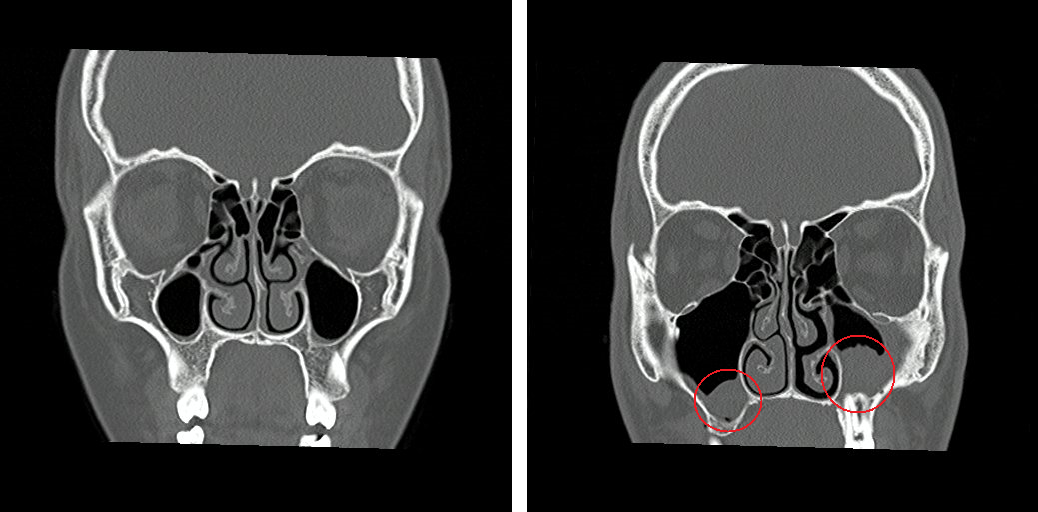
\includegraphics[width=0.8\textwidth]{./Figuras/anomalies.png}
		\caption {Tomografía de cabeza, a la izquierda senos maxilares libres, a la derecha senos maxilares ocupados.}
		\label{fig:anomalies}
		\end{figure}
\end{consigna}

Este tipo de solución permitirá mayor rapidez y exactitud en el diagnóstico de dichas patologías, 
además de permitir la automatización del estudio estadístico en la ocurrencia de estos.

En la figura \ref{fig:diagBloques} se presenta el diagrama de flujo del procedimiento para el 
diagnóstico del paciente con la herramienta que se desarrollará. El primer paso es realizar el
estudio que genera la imagen médica, ya sea una resonancia o una tomografía. A continuación esta 
es procesada por el algoritmo utilizando IA para que finalmente el médico analice los resultados 
obtenidos y pueda así elegir el mejor tratamiento para el paciente.

\begin{consigna}{red}

\begin{figure}[hp]
\centering 
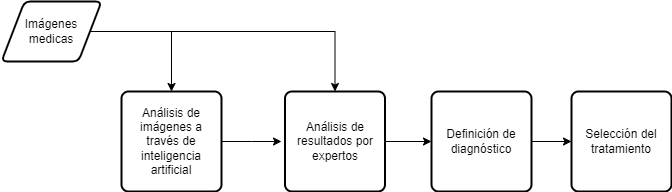
\includegraphics[width=\textwidth]{./Figuras/diagBloques.png}
\caption{Diagrama de flujo para el diagnóstico por imágenes.}
\label{fig:diagBloques}
\end{figure}
\end{consigna}

El proyecto permitirá mejorar la detección temprana de patologías en imágenes médicas de cabeza, 
buscando diagnósticos más rápidos y precisos, para finalmente obtener tratamientos más efectivos. 
Esto no solo mejora la atención al paciente sino que también puede reducir costos médicos 
y mejorar los resultados en salud.


\section{2. Identificación y análisis de los interesados}
\label{sec:interesados}

\begin{consigna}{red} 

\begin{table}[ht]
%\caption{Identificación de los interesados}
%\label{tab:interesados}
\begin{tabularx}{\linewidth}{@{}|l|X|X|l|@{}}
\hline
\rowcolor[HTML]{C0C0C0} 
Rol           & Nombre y Apellido & Organización 	& Puesto 	\\ \hline
%Auspiciante   &                   &              	& -       	\\ \hline
Cliente       & \clientename      &\empclientename	& Médico otorrinolaringólogo       	\\ \hline
%Impulsor      &                   &              	& -       	\\ \hline
Responsable   & \authorname       & FIUBA        	& Alumno 	\\ \hline
%Colaboradores & \clientename	  & \empclientename 	& -       	\\ \hline
Orientador    & \supname	      & \pertesupname 	& Director Trabajo final \\ \hline
%Equipo        & miembro1 \newline 
%				miembro2          &              	&        	\\ \hline
%Opositores    &                   &              	&        	\\ \hline
%Usuario final &  \clientename      &\empclientename	& -       	\\ \hline
\end{tabularx}
\end{table}

\end{consigna} 

\begin{itemize}
	\item Cliente/Colaborador: es un profesional de la salud en el área de otorrinolaringología.
	\item Orientador: \supname, es un especialista en el área de inteligencia artificial y 
	posee experiencia profesional en proyecto de clasificación de objetos en imágenes.
\end{itemize}




\section{3. Propósito del proyecto}
\label{sec:proposito}

El objetivo de este proyecto es desarrollar un algoritmo de inteligencia artificial que emplea el procesamiento  
de imágenes médicas para identificar patologías presentes en radiografías o tomografías de cabeza. El propósito es 
asistir a los médicos en el análisis de este tipo de imágenes, reducir la posibilidad de que se generen errores  
de diagnóstico y finalmente se escoja un tratamiento que solucione la afección del paciente. 

\section{4. Alcance del proyecto}
\label{sec:alcance}

Este proyecto contempla el desarrollo de un algoritmo de inteligencia artificial que permita detectar patologías en 
tomografías de cabeza, con orientación frontal, a través del procesamiento de las imágenes. Su alcance se limita al 
desarrollo del modelo y del pipeline para la preparación del dataset (imágenes y datos médicos). 

Este proyecto no contempla la detección de patologías en imágenes médicas con una orientación diferente a la 
definida o de otras partes del cuerpo, tampoco el despliegue de esta herramienta para su uso.

En cuanto a los entregables se realizará la entrega del análisis de los resultados obtenidos, arquitecturas de  
redes utilizadas, métodos de optimización y evaluación de performance. Solo se hará entrega de datasets utilizados 
que sean de acceso público y no se entregará el modelo final obtenido.


\section{5. Supuestos del proyecto}
\label{sec:supuestos}

Para el desarrollo del presente proyecto se supone que:

\begin{itemize}
	\item Se contará con la disponibilidad de un tiempo de dedicación aproximado de 600 h.
	\item Se contará con el dataset mínimo necesario para el entrenamiento de la inteligencia
	artificial.
	\item Se contará con la colaboración de un médico y de un especialista en inteligencia artificial
	para subsanar dudas y dificultades que puedan encontrarse.
	\item El uso de recursos computacionales se ejecutará utilizando Visual Studio Code.
	\item No se trabajará en el despliegue de la solución para su uso. Se mantendrá la aplicación
	en un entorno controlado de desarrollo.
\end{itemize}


\section{6. Requerimientos}
\label{sec:requerimientos}

Los requerimientos contemplados en el presente proyecto son:

\begin{enumerate}
	\item Requerimientos funcionales:
		\begin{enumerate}
			\item El sistema procesará todas las imágenes que conforman la tomografía.
			\item El modelo entrenado deberá devolver la patología detectada mostrando el área de la imagen 
			donde se lo detectó.
			\item El algoritmo deberá proteger cualquier tipo de información sensible que se maneje en este tipo de estudios.
		\end{enumerate}
	\item Requerimiento de imágenes:
		\begin{enumerate}
			\item 	Se debe tener en cuenta que el entrenamiento se llevará a cabo utilizando imágenes de una determinada calidad, 
					si se utiliza este algoritmo para el análisis de imágenes con una calidad inferior, la precisión de esta 
					herramienta puede ser considerablemente menor a los resultados obtenidos en su desarrollo.
		\end{enumerate}
	\item Requerimientos de documentación:
		\begin{enumerate}
			\item Se conformará un registro del desarrollo realizado incluyendo metodologías, problemas encontrados y resultados.
		\end{enumerate}
	\item Requerimiento de testing:
		\begin{enumerate}
			\item El testeo final del algoritmo se llevará a cabo con el profesional de la salud especializado en las patologías detectadas.
		\end{enumerate}
	


		Se debe tener en cuenta que el entrenamiento se llevará a cabo utilizando imágenes de una determinada calidad, 
		si se utiliza este algoritmo para el análisis de imágenes con una calidad inferior, la precisión de esta 
		herramienta puede ser considerablemente menor a los resultados obtenidos en su desarrollo.


\end{enumerate}


\section{7. Historias de usuarios (\textit{Product backlog})}
\label{sec:backlog}

El criterio para calcular los \textit{story points} de una historia de usuario consiste en analizarla en función de tres criterios:
\begin{itemize}
	\item \textbf{Dificultad:} evalúa el tiempo que puede tomar realizar una tarea.
	\item \textbf{Complejidad:} evalúa qué tan sofisticada puede llegar a ser una tarea.
	\item \textbf{Incertidumbre:} evalúa el riesgo que implica realizar una tarea.
\end{itemize}

El puntaje de cada criterio será un número entero que pertenezca a la sucesión de Fibonacci.
El peso total de cada historia será la suma de cada criterio. En caso de que la suma no sea un
número de la sucesión, se aproximará al número mayor más cercano de ésta. Los puntajes que
fueron asignados son los siguientes:

\begin{table}[H]
	\centering
	\begin{tabularx}{0.57\linewidth}{@{}|X|c|c|c|@{}}
	\hline
	\rowcolor[HTML]{C0C0C0} 
	Valor         & Dificultad & Complejidad & Incertidumbre 	\\ \hline
	Bajo		  &     1      &     1 		 &        1      	\\ \hline
	Medio         & 	3	   &  	 5		 &     	  5     	\\ \hline
	Alto	      &     5      &     8       &  	  8			\\ \hline
	\end{tabularx}
\end{table}


Historia 1:
\begin{itemize}
	\item \textbf{Médico otorrinolaringólogo:} como médico quiero reducir la posibilidad de error en el diagnóstico de patologías 
para elegir el mejor tratamiento para mis pacientes.
\end{itemize}

\begin{itemize}
	\item \textbf{Dificultad:} baja (3). El análisis de las imágenes médicas por partes de un profesional entrenado es una tarea
	sistémica.
	\item \textbf{Complejidad:} alta (8). Garantizar un diagnóstico con total seguridad puede ser un desafío ya que puede haber manchas
	en la imagen producto de cuerpos extraños, anomalías propias de cada individuo, etc.
	\item \textbf{Incertidumbre:} alta (8). Un mal diagnóstico puede causar que se someta al paciente a un tratamiento que no solucione
	 su afección y pueda tener consecuencias graves.
\end{itemize}

Puntaje total en la escala de Fibonacci: 3 + 8 + 8 = 19, como este no es un valor de la escala el mayor siguiente es: \textbf{21}.

Historia 2:
\begin{itemize}
	\item \textbf{Jefe del departamento de otorrinolaringología:} como jefe del departamento quiero automatizar los 
	informes estadísticos de las afecciones más comunes entre los pacientes que se atienden en nuestra institución.
\end{itemize}

\begin{itemize}
	\item \textbf{Dificultad:} alta(5). Juntar los resultados de cientos de pacientes para hacer un estudio estadístico es
	una tarea que lleva tiempo ya que se requiere revisar uno por uno los informes.
	\item \textbf{Complejidad:} baja (1). Realizar un estudio estadístico de los informes ya realizados no es una tarea 
	compleja.
	\item \textbf{Incertidumbre:} medio (5). Estos informes ayudan a realizar tareas de prevención para la salud y dan 
	una noción de que tan grave puede ser la situación social referida a dicha afecciones.
\end{itemize}

Puntaje total en la escala de Fibonacci: 5 + 1 + 5 = 11, como este no es un valor de la escala el mayor siguiente es: \textbf{13}.


\section{8. Entregables principales del proyecto}
\label{sec:entregables}

Los entregables del proyecto son (ejemplo):

\begin{itemize}
	\item Planificación del proyecto.
	\item Documentación sobre el desarrollo.
	\item Datasets de orig
	\item Análisis de performance.
	\item Informe final.
\end{itemize}

\section{9. Desglose del trabajo en tareas}
\label{sec:wbs}

\begin{enumerate}
	\item Planificación (30 h):
		\begin{enumerate}
		\item Elaboración de la planificación del proyecto (20 h).
		\item Revisión de la planificación (5 h).
		\item Presentación de la planificación (5 h).
		\end{enumerate}
	\item Investigación (40 h):
		\begin{enumerate}
		\item Búsqueda y lectura de papers relacionados (40 h).
		\end{enumerate}
	\item Tareas con el dataset (235 h):
		\begin{enumerate}
		\item Recopilación de imágenes (10 h).
		\item Estudio del formato dicom (20 h).
		\item Adecuación de las imágenes (40 h).
		\item Búsqueda de datasets de acceso público (tantas 15 h).
		\item Etiquetado de imágenes (150 h).
		\end{enumerate}
	\item Desarrollo (220 h):
		\begin{enumerate}
		\item Desarrollo de código (120 h).
		\item Entrenamiento de la IA (80 h).
		\item Evaluación de resultados (20 h).
		\end{enumerate}
	\item Documentacion (80 h):
		\begin{enumerate}
		\item Escritura de informe de avances (10 h).
		\item Documentación del trabajo (20 h).
		\item Confección del informe del trabajo final (40 h).
		\item Presentación final (10 h).
		\end{enumerate}
	\end{enumerate}

Cantidad total de horas: (605 h).

\section{10. Diagrama de Activity On Node}
\label{sec:AoN}

En la figura \ref{fig:AoNRef} se muestran las referencias del diagrama de \textit{Activity on Node}

\begin{figure}[htpb]
	\centering 
	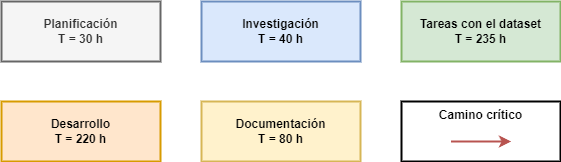
\includegraphics[width=.7\textwidth]{./Figuras/AoNReferences.png}
	\caption{Referencias del diagrama de \textit{Activity on Node}.}
	\label{fig:AoNRef}
\end{figure}

La figura \ref{fig:AoN} muestra el diagrama de Activity on Node donde se describen las duraciones
y dependencias de las actividades para el desarrollo del presente trabajo. Se utilizaron flechas
rojas para indicar el camino crítico, se calculó la duración de este camino en 555 h.


\begin{figure}[htpb]
\centering 
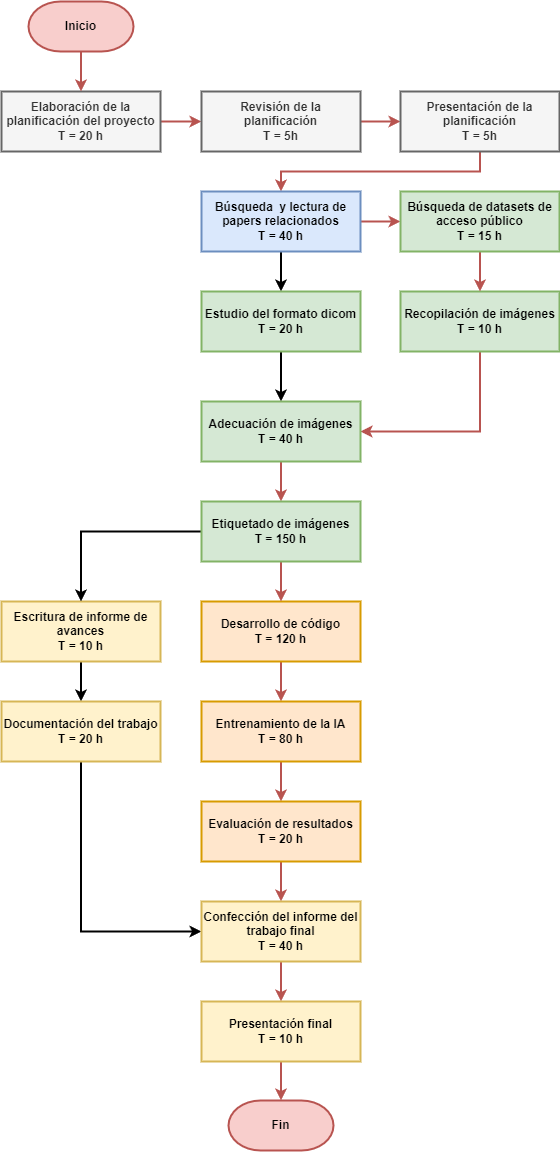
\includegraphics[width=.7\textwidth]{./Figuras/ActivityonNode.png}
\caption{Diagrama de \textit{Activity on Node}.}
\label{fig:AoN}
\end{figure}


\section{11. Diagrama de Gantt}
\label{sec:gantt}


%\begin{landscape}
\begin{figure}[htpb]
\centering 
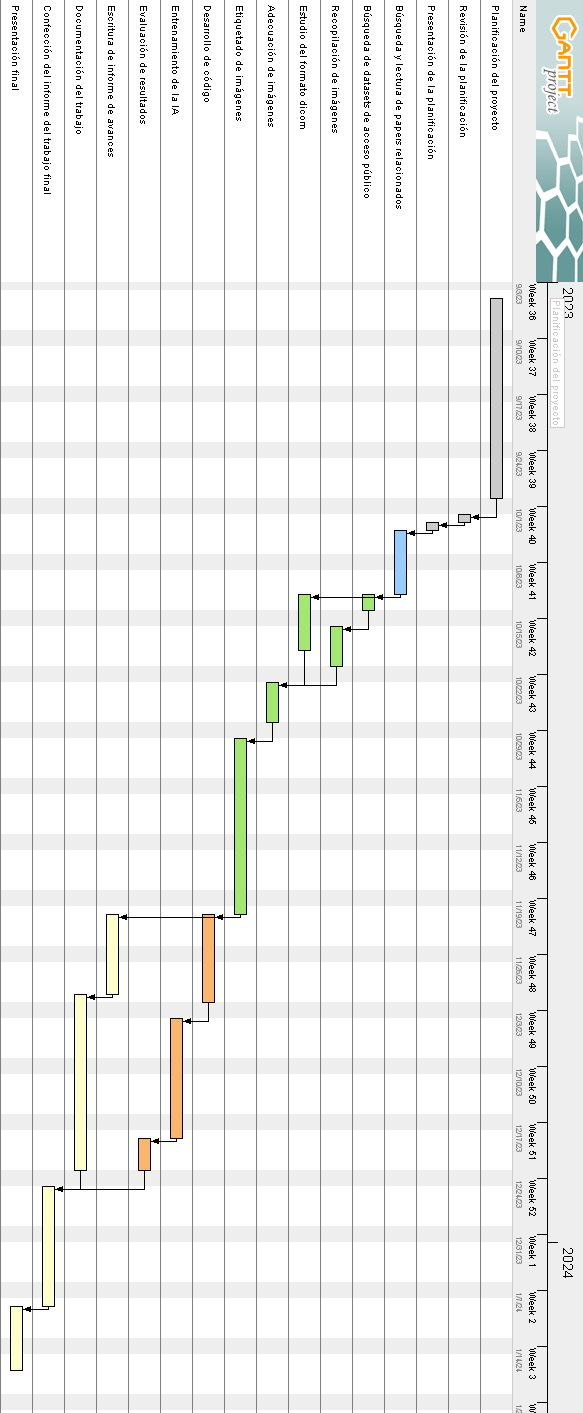
\includegraphics[height=.74\textheight]{./Figuras/GANTCEIA.png}
\caption{Diagrama de Gantt.}
\label{fig:diagGantt}
\end{figure}

%\end{landscape}


\section{12. Presupuesto detallado del proyecto}
\label{sec:presupuesto}

En la siguiente tabla se detalla el presupuesto del proyecto en dólares estadounidenses.
Se considera la compra de una computadora para el desarrollo del proyecto y los gastos de 
servicios necesarios.

\begin{table}[htpb]
\centering
\begin{tabularx}{\linewidth}{@{}|X|c|r|r|@{}}
\hline
\rowcolor[HTML]{C0C0C0} 
\multicolumn{4}{|c|}{\cellcolor[HTML]{C0C0C0}COSTOS DIRECTOS} \\ \hline
\rowcolor[HTML]{C0C0C0} 
Descripción &
  \multicolumn{1}{c|}{\cellcolor[HTML]{C0C0C0}Cantidad} &
  \multicolumn{1}{c|}{\cellcolor[HTML]{C0C0C0}Valor unitario} &
  \multicolumn{1}{c|}{\cellcolor[HTML]{C0C0C0}Valor total} \\ \hline
Horas laborales &
  \multicolumn{1}{c|}{605} &
  \multicolumn{1}{c|}{\$10} &
  \multicolumn{1}{c|}{\$6050} \\ \hline
Compra de computadora dedicada &
  \multicolumn{1}{c|}{1} &
  \multicolumn{1}{c|}{\$1500} &
  \multicolumn{1}{c|}{\$1500} \\ \hline

\multicolumn{3}{|c|}{SUBTOTAL} &
  \multicolumn{1}{c|}{\$7550} \\ \hline
\rowcolor[HTML]{C0C0C0} 
\multicolumn{4}{|c|}{\cellcolor[HTML]{C0C0C0}COSTOS INDIRECTOS} \\ \hline
\rowcolor[HTML]{C0C0C0} 
Descripción &
  \multicolumn{1}{c|}{\cellcolor[HTML]{C0C0C0}Cantidad} &
  \multicolumn{1}{c|}{\cellcolor[HTML]{C0C0C0}Valor unitario} &
  \multicolumn{1}{c|}{\cellcolor[HTML]{C0C0C0}Valor total} \\ \hline
Servicio de internet &
	\multicolumn{1}{c|}{8 meses} &
	\multicolumn{1}{c|}{\$5} &
	\multicolumn{1}{c|}{\$40} \\ \hline
Servicio electrico &
	\multicolumn{1}{c|}{8 meses} &
	\multicolumn{1}{c|}{\$15} &
	\multicolumn{1}{c|}{\$120} \\ \hline
\multicolumn{3}{|c|}{SUBTOTAL} &
  \multicolumn{1}{c|}{\$160} \\ \hline
\rowcolor[HTML]{C0C0C0}
\multicolumn{3}{|c|}{TOTAL} &
	\multicolumn{1}{c|}{\$7710}\\ \hline
\end{tabularx}%
\end{table}


\section{13. Gestión de riesgos}
\label{sec:riesgos}

\begin{consigna}{red}
a) Identificación de los riesgos (al menos cinco) y estimación de sus consecuencias:
 
Riesgo 1: detallar el riesgo (riesgo es algo que si ocurre altera los planes previstos de forma negativa)
\begin{itemize}
	\item Severidad (S): mientras más severo, más alto es el número (usar números del 1 al 10).\\
	Justificar el motivo por el cual se asigna determinado número de severidad (S).
	\item Probabilidad de ocurrencia (O): mientras más probable, más alto es el número (usar del 1 al 10).\\
	Justificar el motivo por el cual se asigna determinado número de (O). 
\end{itemize}   

Riesgo 2:
\begin{itemize}
	\item Severidad (S): 
	\item Ocurrencia (O):
\end{itemize}

Riesgo 3:
\begin{itemize}
	\item Severidad (S): 
	\item Ocurrencia (O):
\end{itemize}


b) Tabla de gestión de riesgos:      (El RPN se calcula como RPN=SxO)

\begin{table}[htpb]
\centering
\begin{tabularx}{\linewidth}{@{}|X|c|c|c|c|c|c|@{}}
\hline
\rowcolor[HTML]{C0C0C0} 
Riesgo & S & O & RPN & S* & O* & RPN* \\ \hline
       &   &   &     &    &    &      \\ \hline
       &   &   &     &    &    &      \\ \hline
       &   &   &     &    &    &      \\ \hline
       &   &   &     &    &    &      \\ \hline
       &   &   &     &    &    &      \\ \hline
\end{tabularx}%
\end{table}

Criterio adoptado: 
Se tomarán medidas de mitigación en los riesgos cuyos números de RPN sean mayores a...

Nota: los valores marcados con (*) en la tabla corresponden luego de haber aplicado la mitigación.

c) Plan de mitigación de los riesgos que originalmente excedían el RPN máximo establecido:
 
Riesgo 1: plan de mitigación (si por el RPN fuera necesario elaborar un plan de mitigación).
  Nueva asignación de S y O, con su respectiva justificación:
  - Severidad (S): mientras más severo, más alto es el número (usar números del 1 al 10).
          Justificar el motivo por el cual se asigna determinado número de severidad (S).
  - Probabilidad de ocurrencia (O): mientras más probable, más alto es el número (usar del 1 al 10).
          Justificar el motivo por el cual se asigna determinado número de (O).

Riesgo 2: plan de mitigación (si por el RPN fuera necesario elaborar un plan de mitigación).
 
Riesgo 3: plan de mitigación (si por el RPN fuera necesario elaborar un plan de mitigación).

\end{consigna}


\section{14. Gestión de la calidad}
\label{sec:calidad}

\begin{consigna}{red}
Elija al menos diez requerientos que a su criterio sean los más importantes/críticos/que aportan más valor y para cada uno de ellos indique las acciones de verificación y validación que permitan asegurar su cumplimiento.

\begin{itemize} 
\item Req \#1: copiar acá el requerimiento.

\begin{itemize}
	\item Verificación para confirmar si se cumplió con lo requerido antes de mostrar el sistema al cliente. Detallar 
	\item Validación con el cliente para confirmar que está de acuerdo en que se cumplió con lo requerido. Detallar  
\end{itemize}

\end{itemize}

Tener en cuenta que en este contexto se pueden mencionar simulaciones, cálculos, revisión de hojas de datos, consulta con expertos, mediciones, etc.  Las acciones de verificación suelen considerar al entregable como ``caja blanca'', es decir se conoce en profundidad su funcionamiento interno.  En cambio, las acciones de validación suelen considerar al entregable como ``caja negra'', es decir, que no se conocen los detalles de su funcionamiento interno.

\end{consigna}

\section{15. Procesos de cierre}    
\label{sec:cierre}

\begin{consigna}{red}
Establecer las pautas de trabajo para realizar una reunión final de evaluación del proyecto, tal que contemple las siguientes actividades:

\begin{itemize}
	\item Pautas de trabajo que se seguirán para analizar si se respetó el Plan de Proyecto original:
	 - Indicar quién se ocupará de hacer esto y cuál será el procedimiento a aplicar. 
	\item Identificación de las técnicas y procedimientos útiles e inútiles que se emplearon, y los problemas que surgieron y cómo se solucionaron:
	 - Indicar quién se ocupará de hacer esto y cuál será el procedimiento para dejar registro.
	\item Indicar quién organizará el acto de agradecimiento a todos los interesados, y en especial al equipo de trabajo y colaboradores:
	  - Indicar esto y quién financiará los gastos correspondientes.
\end{itemize}

\end{consigna}


\end{document}
